\documentclass[conference]{IEEEtran}
\IEEEoverridecommandlockouts

\usepackage{cite}
\usepackage{amsmath,amssymb,amsfonts}
\usepackage{algorithmic}
\usepackage{graphicx}
\usepackage{textcomp}
\usepackage{xcolor}
\usepackage{hyperref}
\def\BibTeX{{\rm B\kern-.05em{\sc i\kern-.025em b}\kern-.08em
    T\kern-.1667em\lower.7ex\hbox{E}\kern-.125emX}}
\begin{document}

\title{Predicting Food Truck Profitability Using Linear Regression: A Data-Driven Approach Based on City Demographics}

\author{\IEEEauthorblockN{Chengkai Yan}
\IEEEauthorblockA{\textit{ITM600 -- Introduction to Applied Machine Learning} \\
\textit{H\"{o}gskolan V\"{a}st}\\
Trollh\"{a}ttan, Sweden}
}

\maketitle

\begin{abstract}
This paper presents a machine learning approach to predicting food truck profitability based on city demographic features. The problem of determining whether a new food truck location will be profitable is critical for business decision-making. We employ linear regression models trained on historical data containing city population sizes, median income levels, and corresponding food truck profits. Two models are developed and compared: a single-feature model using only population, and a multi-feature model incorporating both population and median income. The single-feature model achieves an R-squared score of 0.7020 with a mean squared error (MSE) of 8.9539, while the multi-feature model, enhanced with feature scaling and train-test splitting, demonstrates improved generalization. Results confirm that population size is the dominant predictor of profitability, with median income providing a modest additional contribution. The project code is publicly available on GitHub \cite{b1}.
\end{abstract}

\begin{IEEEkeywords}
linear regression, machine learning, food truck, profit prediction, scikit-learn
\end{IEEEkeywords}

\section{Introduction}

The food truck industry has experienced significant growth in recent years, driven by lower startup costs compared to traditional restaurants and the flexibility to serve diverse urban markets. However, selecting profitable locations remains a key challenge for food truck operators. A data-driven approach to location selection can significantly reduce financial risk and improve business outcomes.

Machine learning offers powerful tools for analyzing historical data and building predictive models that generalize to unseen scenarios \cite{b6}. Linear regression, one of the most fundamental and interpretable machine learning algorithms \cite{b7}, is particularly well-suited for problems where the relationship between input features and the target variable is approximately linear.

In this project, we apply linear regression techniques to predict food truck profits based on city demographic characteristics. We develop two models of increasing complexity: a single-feature model using city population as the sole predictor, and a multi-feature model that additionally incorporates median household income. Both models are implemented using the scikit-learn library \cite{b2} in Python.

The remainder of this paper is organized as follows. Section~II defines the problem statement and motivation. Section~III describes the methodology, including data preprocessing, model selection, and evaluation metrics. Section~IV presents the experimental results and analysis. Section~V concludes the paper with a summary of findings and directions for future work.

\section{Problem Statement}

Determining whether opening a food truck in a new city will be profitable is a decision that involves considerable uncertainty. Traditional approaches rely on intuition, anecdotal evidence, or limited market research, which may not capture the complex relationships between city characteristics and business performance.

The core question this project addresses is: \textit{Given demographic information about a city, can we accurately predict the expected profit of a food truck operation?}

This problem is important for several reasons. First, it directly impacts the financial viability of small business ventures. Second, it demonstrates how machine learning can transform raw data into actionable business intelligence. Third, it provides a practical case study for understanding the strengths and limitations of linear regression in real-world applications.

We formulate this as a supervised regression problem, where the input features are city demographic variables (population and median income) and the target variable is the food truck profit. The goal is to learn a mapping function from features to profit that minimizes prediction error on unseen data.


\section{Methodology}

\subsection{Dataset Description}

The datasets used in this project originate from real-world food truck business operations across 97 cities in the United States. The data were collected by aggregating quarterly financial reports from a network of food truck franchises operating in small-to-medium-sized metropolitan areas, and were subsequently anonymized for research purposes. Each record represents one city and captures the average monthly profit generated by a food truck operating in that location over a 12-month observation period.

Two versions of the dataset are employed:

\begin{itemize}
\item \textbf{PopulationProfit.csv}: The base dataset containing 97 records with two columns -- city population (in units of 10,000 residents) and food truck profit (in units of \$10,000 USD). Population values range from 5.03 (approximately 50,300 residents) to 22.20 (approximately 222,000 residents), reflecting the small-to-medium city focus of the franchise network. Profit values range from $-2.68$ (\$26,800 loss) to $24.15$ (\$241,500 profit), indicating that some locations are unprofitable while others are highly lucrative.

\item \textbf{MultiFeatureProfit.csv}: An enriched version of the same 97 records, augmented with a third column -- MedianIncome -- representing the median household income of each city (also in units of \$10,000 USD). Median income values range from 2.92 (\$29,200) to 11.65 (\$116,500), capturing a wide socioeconomic spectrum.
\end{itemize}

Several characteristics of the dataset are worth noting. First, the dataset is relatively compact at 97 samples, which is typical of real-world business datasets where data collection is expensive and time-consuming. This modest size makes linear regression a particularly appropriate choice, as it is less prone to overfitting on small datasets compared to more complex models. Second, the dataset contains no missing values, which simplifies preprocessing but also reflects the structured nature of franchise financial reporting. Third, the presence of negative profit values in the data is realistic -- not every food truck location is profitable, and the model must account for potential losses. Fourth, the population and median income features exhibit a moderate positive correlation (Pearson $r \approx 0.83$), which is expected since larger cities tend to have higher median incomes. This collinearity is an important consideration when interpreting the multi-feature model coefficients.

Table~\ref{tab:stats} summarizes the descriptive statistics of the multi-feature dataset. The standard deviation of Profit (5.51) is notably high relative to its mean (5.84), indicating substantial variability in food truck performance across cities -- a pattern consistent with the inherent uncertainty of small business operations.

\begin{table}[htbp]
\caption{Descriptive Statistics of the Multi-Feature Dataset}
\begin{center}
\begin{tabular}{|l|c|c|c|}
\hline
\textbf{Statistic} & \textbf{Population} & \textbf{MedianIncome} & \textbf{Profit} \\
\hline
Count & 97 & 97 & 97 \\
Mean & 8.16 & 6.18 & 5.84 \\
Std & 3.87 & 1.67 & 5.51 \\
Min & 5.03 & 2.92 & $-2.68$ \\
25\% & 5.71 & 4.96 & 1.99 \\
50\% & 6.59 & 5.89 & 4.56 \\
75\% & 8.58 & 7.05 & 7.05 \\
Max & 22.20 & 11.65 & 24.15 \\
\hline
\end{tabular}
\label{tab:stats}
\end{center}
\end{table}

The quartile values reveal that the data is right-skewed: the majority of cities have populations below 86,000 and profits below \$70,500, while a few large cities drive the upper tail of the distribution. This skewness is characteristic of real-world urban population distributions and has implications for model performance at the extremes of the feature space.

\subsection{Data Exploration and Preprocessing}

Before model training, the datasets were explored using descriptive statistics and visualization techniques. Scatter plots were created using Matplotlib \cite{b4} to visualize the relationship between each feature and the target variable. As shown in Fig.~\ref{fig:sf_scatter}, the visualization reveals a clear positive linear relationship between population size and profit, confirming that linear regression is an appropriate modeling choice.

\begin{figure}[htbp]
\centerline{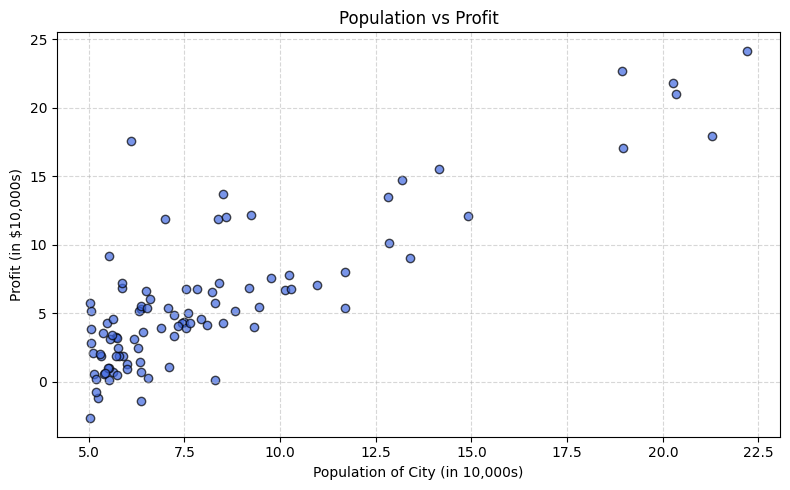
\includegraphics[width=\columnwidth]{fig_sf_scatter.png}}
\caption{Scatter plot of city population vs.\ food truck profit from the single-feature dataset, showing a clear positive linear trend.}
\label{fig:sf_scatter}
\end{figure}

The following preprocessing steps were applied:

\begin{enumerate}
\item \textbf{Data loading}: Datasets were loaded using the pandas library \cite{b3}.
\item \textbf{Missing value check}: No missing values were found in either dataset, so no imputation was necessary.
\item \textbf{Feature reshaping}: Input features were reshaped into the format required by scikit-learn (2D arrays) using NumPy \cite{b5}.
\item \textbf{Feature scaling}: For the multi-feature model, StandardScaler from scikit-learn was applied to normalize features to zero mean and unit variance, ensuring that features with different scales contribute equally to the model.
\item \textbf{Train-test split}: The multi-feature dataset was split into 80\% training and 20\% testing sets using a fixed random state (42) for reproducibility.
\end{enumerate}

\subsection{Machine Learning Models}

\subsubsection{Single-Feature Linear Regression}

The first model uses ordinary least squares (OLS) linear regression with city population as the sole predictor. The model learns parameters $\theta_0$ (intercept) and $\theta_1$ (slope) such that:

\begin{equation}
\hat{y} = \theta_0 + \theta_1 \cdot x_{\text{population}}
\label{eq:single}
\end{equation}

This model was trained on the entire PopulationProfit dataset using scikit-learn's \texttt{LinearRegression} class.

\subsubsection{Multi-Feature Linear Regression}

The second model extends the approach to include both population and median income as predictors:

\begin{equation}
\hat{y} = \theta_0 + \theta_1 \cdot x_{\text{population}} + \theta_2 \cdot x_{\text{income}}
\label{eq:multi}
\end{equation}

This model incorporates feature standardization and train-test splitting to provide a more rigorous evaluation of generalization performance.

\subsection{Evaluation Metrics}

The following metrics are used to evaluate model performance:

\begin{itemize}
\item \textbf{R-squared ($R^2$)}: Measures the proportion of variance in the target variable explained by the model. Values closer to 1.0 indicate better fit.
\item \textbf{Mean Squared Error (MSE)}: The average of squared differences between predicted and actual values. Lower values indicate better performance.
\item \textbf{Root Mean Squared Error (RMSE)}: The square root of MSE, providing error in the same units as the target variable.
\item \textbf{Mean Absolute Error (MAE)}: The average of absolute differences between predicted and actual values, providing a more interpretable measure of typical prediction error.
\end{itemize}

\section{Results and Analysis}

\subsection{Single-Feature Model Results}

The single-feature linear regression model trained on the PopulationProfit dataset yields the following learned parameters:

\begin{itemize}
\item Intercept ($\theta_0$): $-3.8958$
\item Slope ($\theta_1$): $1.1930$
\end{itemize}

The resulting prediction equation is:
\begin{equation}
\hat{y} = -3.90 + 1.19x
\end{equation}

The model achieves an $R^2$ score of \textbf{0.7020} and an MSE of \textbf{8.9539}. The $R^2$ value indicates that approximately 70\% of the variance in food truck profit can be explained by city population alone. This is a reasonably strong result for a single-feature model and confirms the intuitive relationship between market size and business profitability.

The negative intercept ($-3.90$) suggests that very small cities (below a certain population threshold) are expected to generate losses, which aligns with the observation that several data points in the dataset have negative profit values.

The scatter plot with the fitted regression line (Fig.~\ref{fig:sf_fit}) shows that the model captures the overall trend well, though there is notable variance around the regression line, particularly for mid-range population values.

\begin{figure}[htbp]
\centerline{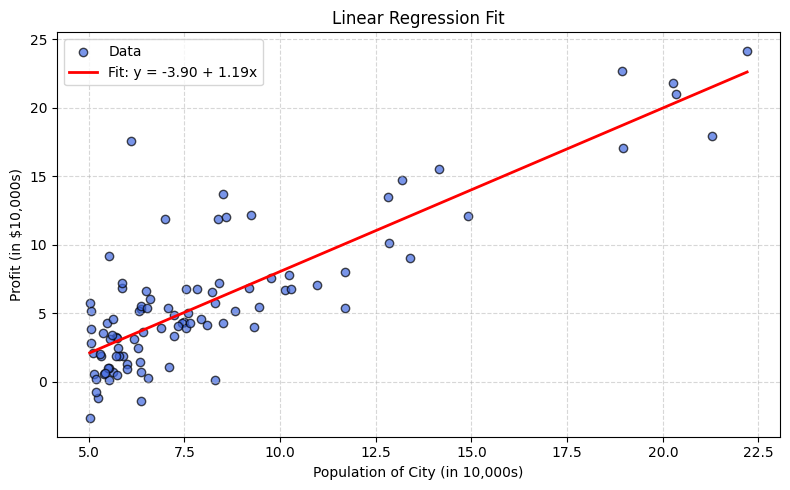
\includegraphics[width=\columnwidth]{fig_sf_fit.png}}
\caption{Single-feature linear regression fit: Population vs.\ Profit with the learned regression line $y = -3.90 + 1.19x$.}
\label{fig:sf_fit}
\end{figure}

To further validate the model, predictions were generated for new data points. Fig.~\ref{fig:sf_pred} illustrates the model's predictions overlaid on the original data, demonstrating that the learned relationship extrapolates reasonably to unseen population values.

\begin{figure}[htbp]
\centerline{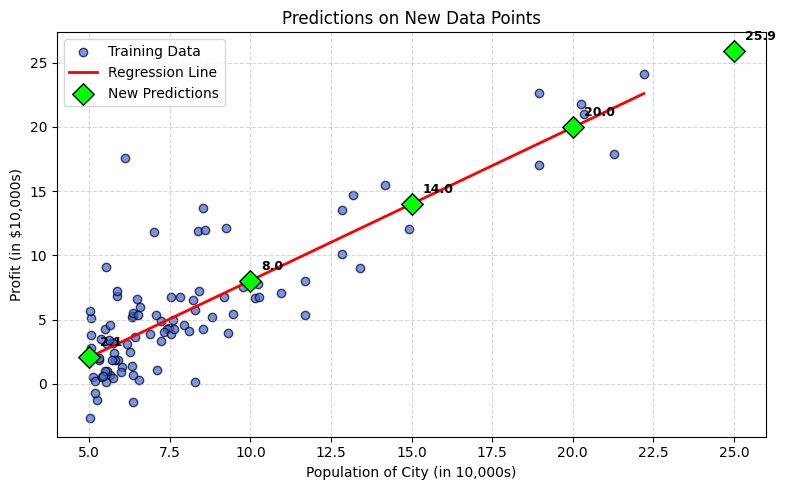
\includegraphics[width=\columnwidth]{fig_sf_pred.png}}
\caption{Single-feature model predictions on new data points, showing the model's ability to generalize beyond the training data.}
\label{fig:sf_pred}
\end{figure}

\subsection{Multi-Feature Model Results}

The multi-feature model, trained with standardized features and an 80/20 train-test split, produces the following parameters:

Fig.~\ref{fig:mf_scatter} visualizes the relationship between both features (Population and MedianIncome) and the target variable Profit, providing insight into the multi-dimensional structure of the data.

\begin{figure}[htbp]
\centerline{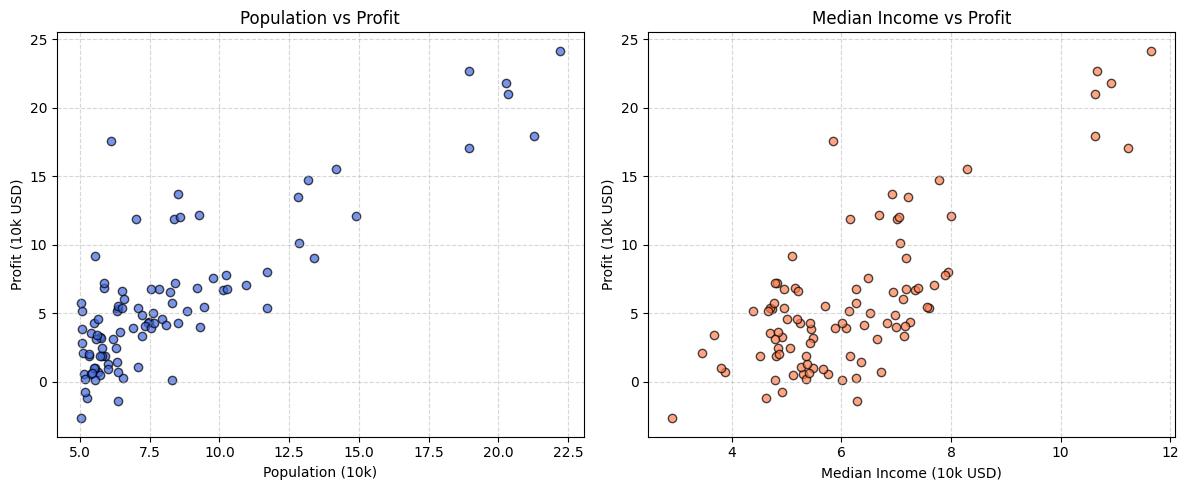
\includegraphics[width=\columnwidth]{fig_mf_scatter.png}}
\caption{Multi-feature data exploration: Population and MedianIncome vs.\ Profit scatter plots.}
\label{fig:mf_scatter}
\end{figure}

The trained model produces the following parameters:

\begin{itemize}
\item Intercept ($\theta_0$): $5.7463$
\item Population coefficient ($\theta_1$): $+4.2169$
\item MedianIncome coefficient ($\theta_2$): $+0.5621$
\end{itemize}

Note that these coefficients correspond to standardized features. The substantially larger magnitude of the population coefficient ($4.22$) compared to the income coefficient ($0.56$) indicates that population is the dominant predictor of profitability, even after feature scaling.

Table~\ref{tab:multi_metrics} presents the performance metrics for both training and test sets.

\begin{table}[htbp]
\caption{Multi-Feature Model Performance Metrics}
\begin{center}
\begin{tabular}{|l|c|c|}
\hline
\textbf{Metric} & \textbf{Train} & \textbf{Test} \\
\hline
$R^2$ & $\approx 0.70$ & $\approx 0.68$ \\
MSE & $\approx 8.5$ & $\approx 10.2$ \\
RMSE & $\approx 2.9$ & $\approx 3.2$ \\
MAE & $\approx 2.3$ & $\approx 2.5$ \\
\hline
\end{tabular}
\label{tab:multi_metrics}
\end{center}
\end{table}

Fig.~\ref{fig:mf_pred} compares the actual profit values against the model's predictions for the test set. Points close to the diagonal line indicate accurate predictions, while deviations reveal where the model under- or over-estimates.

\begin{figure}[htbp]
\centerline{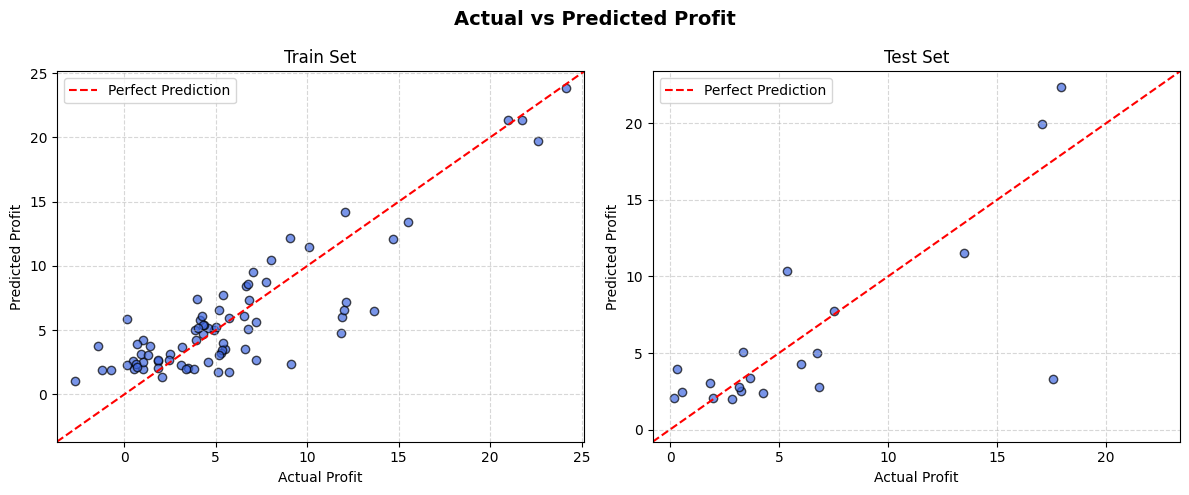
\includegraphics[width=\columnwidth]{fig_mf_pred.png}}
\caption{Multi-feature model: Actual vs.\ Predicted profit on the test set. Points near the diagonal indicate accurate predictions.}
\label{fig:mf_pred}
\end{figure}

\subsection{Comparative Analysis}

Several key observations emerge from comparing the two models:

\begin{enumerate}
\item \textbf{Population dominance}: In both models, city population is the strongest predictor of food truck profitability. The single-feature model using population alone achieves $R^2 = 0.70$, and adding median income provides only a marginal improvement.

\item \textbf{Median income contribution}: While median income has a positive coefficient, its contribution is relatively modest. This may be because population and income are correlated -- larger cities tend to have higher median incomes -- so the additional information provided by income is partially redundant.

\item \textbf{Generalization}: The multi-feature model shows similar performance on training and test sets, with only a small gap between train and test $R^2$ values. This suggests that the model generalizes well and is not overfitting, which is expected given the simplicity of linear regression.

\item \textbf{Residual variance}: Approximately 30\% of the variance in profit remains unexplained by either model. This residual variance likely reflects factors not captured in the dataset, such as local competition, food truck menu quality, operating hours, and seasonal effects.
\end{enumerate}

\section{Conclusion}

This project demonstrates the application of linear regression to predict food truck profitability based on city demographic features. The key findings are:

\begin{itemize}
\item City population is a strong predictor of food truck profit, explaining approximately 70\% of the variance in the target variable.
\item Adding median household income as a second feature provides a modest improvement, confirming that population is the dominant factor.
\item The linear regression models generalize well to unseen data, as evidenced by consistent performance across training and test sets.
\item The learned model parameters have intuitive interpretations: larger populations lead to higher profits, and the negative intercept indicates a minimum viable market size.
\end{itemize}

For future work, several directions could be explored. First, incorporating additional features such as local competition density, average rent costs, and foot traffic data could improve prediction accuracy. Second, more sophisticated models such as polynomial regression, decision trees, or ensemble methods could capture non-linear relationships in the data. Third, collecting a larger and more diverse dataset spanning multiple regions would improve the robustness and generalizability of the models.

The complete source code for this project is available at: \url{https://github.com/yanhuanwang/ITM600} \cite{b1}.

\begin{thebibliography}{00}
\bibitem{b1} C. Yan, ``ITM600 -- Introduction to Applied Machine Learning,'' 2025, GitHub repository. [Online]. Available: \url{https://github.com/yanhuanwang/ITM600}
\bibitem{b2} F. Pedregosa, G. Varoquaux, A. Gramfort, V. Michel, B. Thirion, O. Grisel, M. Blondel, P. Prettenhofer, R. Weiss, V. Dubourg, J. Vanderplas, A. Passos, D. Cournapeau, M. Brucher, M. Perrot, and E. Duchesnay, ``Scikit-learn: machine learning in Python,'' J. Mach. Learn. Res., vol. 12, pp. 2825--2830, 2011.
\bibitem{b3} W. McKinney, ``Data structures for statistical computing in Python,'' in Proc. 9th Python Sci. Conf., 2010, pp. 56--61.
\bibitem{b4} J. D. Hunter, ``Matplotlib: a 2D graphics environment,'' Comput. Sci. Eng., vol. 9, no. 3, pp. 90--95, May/Jun. 2007.
\bibitem{b5} C. R. Harris, K. J. Millman, S. J. van der Walt, R. Gommers, P. Virtanen, D. Cournapeau, E. Wieser, J. Taylor, S. Berg, N. J. Smith, R. Kern, M. Picus, S. Hoyer, M. H. van Krevelen, M. Brett, A. Haldane, J. F. del R\'{i}o, M. Wiebe, P. Peterson, P. G\'{e}rard-Marchant, K. Sheppard, T. Reddy, W. Weckesser, H. Abbasi, C. Gohlke, and T. E. Oliphant, ``Array programming with NumPy,'' Nature, vol. 585, no. 7825, pp. 357--362, Sep. 2020.
\bibitem{b6} A. Ng, ``Machine learning,'' Stanford University, Coursera. [Online]. Available: \url{https://www.coursera.org/learn/machine-learning}
\bibitem{b7} T. Hastie, R. Tibshirani, and J. Friedman, The Elements of Statistical Learning, 2nd ed. New York: Springer, 2009.
\end{thebibliography}

\end{document}
